%% 
%% Copyright 2019 Elsevier Ltd
%% 
%% This file is part of the 'CAS Bundle'.
%% --------------------------------------
%% 
%% It may be distributed under the conditions of the LaTeX Project Public
%% License, either version 1.2 of this license or (at your option) any
%% later version.  The latest version of this license is in
%%    http://www.latex-project.org/lppl.txt
%% and version 1.2 or later is part of all distributions of LaTeX
%% version 1999/12/01 or later.
%% 
%% The list of all files belonging to the 'CAS Bundle' is
%% given in the file `manifest.txt'.
%% 
%% Template article for cas-dc documentclass for 
%% double column output.

%\documentclass[a4paper,fleqn,longmktitle]{cas-dc}
\documentclass[a4paper,fleqn]{cas-dc}

%\usepackage[authoryear,longnamesfirst]{natbib}
%\usepackage[authoryear]{natbib}
\usepackage[numbers]{natbib}
\usepackage{listings}
\usepackage{adjustbox}
\usepackage{cleveref}

%%%Author definitions
\def\tsc#1{\csdef{#1}{\textsc{\lowercase{#1}}\xspace}}
\tsc{WGM}
\tsc{QE}
\tsc{EP}
\tsc{PMS}
\tsc{BEC}
\tsc{DE}
%%%

\begin{document}
\let\WriteBookmarks\relax
\def\floatpagepagefraction{1}
\def\textpagefraction{.001}
\shorttitle{SDN-Based Multidomain Service Provisioning and Topology Visualization}
\shortauthors{S. Barguil et~al.}

\title [mode = title]{SDN-Based Multidomain Service Provisioning and Topology Visualization}                      
%%\tnotemark[1,2]

%%\tnotetext[1]{This document is the results of the research
%%   project funded by the National Science Foundation.}

%%\tnotetext[2]{The second title footnote which is a longer text matter
%%   to fill through the whole text width and overflow into
%%  another line in the footnotes area of the first page.}%%

\author[1,4]{Samier Barguil}[type=editor,bioid=1]
\ead{samier.barguil@estudiante.uam.es}
\cormark[1]

\author[2]{Victor Lopez Alvarez}[bioid=4]
\ead{victor.lopezalvarez@telefonica.com}

\author[4]{Cristyan Manta-Caro}[bioid=2]
\ead{cristyan.manta@wipro.com}

\author[4]{Cristian Rosero-Carvajal}[bioid=3]
\ead{cristian.carvajal@wipro.com}

\author[2]{Arturo Mayoral Lopez De Lerma}[bioid=5]
\ead{arturo.mayoral@telefonica.com}

\author[2]{Oscar Gonzalez De Dios}[bioid=6]
\ead{oscar.gonzalezdedios@telefonica.com}

\author[3]{Edward Echeverry}[bioid=7]
\ead{edward.echeverry@telefonica.com}

\author[2]{Juan Pedro Fernandez-Palacios}[bioid=8]
\ead{juanpedro.fernandez-palaciosgimenez@telefonica.com}

\author[5]{Janne Karvonen}[bioid=10]
\ead{jkarvonen@infinera.com}

\author[5]{Jutta Kemppainen}[bioid=10]
\ead{jkemppainen@infinera.com}

\author[5]{Natalia Maya}[bioid=11]
\ead{nmaya@infinera.com}

\address[1]{Universidad Autonoma de Madrid, Madrid, Spain}
\address[2]{Telefonica I+D, Ronda de la Comunicacion, Madrid, Spain}
\address[3]{Telefonica Movistar, Transversal 60 No 114ª -55. Bogotá, Colombia}
\address[4]{Wipro Technologies Ltd., Doddakannelli, Sarjapur Road
Bengaluru - 560 035, India}
\address[5]{Infinera Corporation, 140 Caspian Court, Sunnyvale, CA 94089, USA}

\cortext[cor1]{Corresponding author}

%%\fntext[fn1]{This is the first author footnote. but is common to third
%%  author as well.}
%%\fntext[fn2]{Another author footnote, this is a very long footnote and
%%  it should be a really long footnote. But this footnote is not yet
%%  sufficiently long enough to make two lines of footnote text.}

%%\nonumnote{This note has no numbers. In this work we demonstrate $a_b$
%%  the formation Y\_1 of a new type of polariton on the interface
%%  between a cuprous oxide slab and a polystyrene micro-sphere placed
%%  on the slab.
%%  }

\begin{abstract}
Software-Defined Networking (SDN) is a powerful paradigm already transforming the everyday operations in Telecommunications Networks. SDN came with the idea of decoupling forwarding and control plane in the switches via OpenFlow, but it has evolved to cope with the needs of production networks. Network operators can not change their footprint to upgrade the entire network to support SDN from scratch. This why network operators adapt the original SDN concept into a hybrid SDN approach to have a pragmatic, evolutionary and economically viable solution. This paper tests an  SDN architecture is based on a hierarchical structure of SDN controllers for each technological domain and a Software-Defined Transport Networking (SDTN) controller, which deals with the end-to-end aspects of the service, topology, performance and inventory aspects. Such hierarchical approach allows a service provider to migrate islands in SDN domains, starting with the abstract programmatic interfaces and, when the devices will support it, program each device with a standard interface. 

Service provisioning is a key process in the value chain for supplying next-generation services to customers of all sizes and characteristics. Commonly, during years service provisioning was executed manually, then supported by service activators tuned tools for the vendor- specific combination of network elements. With the advent boom of SDN, service delivery operations can be performed in an agnostic-vendor fashion using standard data models and protocols. However, new challenges still persist such as orchestrate multiple layers required for covering long-haul, medium and short distances. Multidomain networking between IP/MPLS-based layers and underlying WDM multi-layer technologies require further coordination and orchestration. This presents two use cases to enable multidomain service provisioning and the corresponding topology visualization. Moreover, this work demonstrates the capabilities of a SDTN controller in a field trial environment our approach for Hybrid SDN architectures. 

\end{abstract}

% \begin{graphicalabstract}
% 
\includegraphics{figs/grabs.pdf}
% \end{graphicalabstract}

% \begin{highlights}
% \item Research highlights item 1
% \item Research highlights item 2
% \item Research highlights item 3
% \end{highlights}

\begin{keywords}
Software-Defined Networking,
\sep SDN-based Use Cases, 
\sep Service Provisioning,
\sep Multidomain Topology
\sep Network Modelling, 
\sep YANG,  
\end{keywords}

\maketitle

\section{Introduction}
Software-Defined Networking (SDN) has emerged as the new reference paradigm to promote network automation and programmability. It has promoted the idea of a real transformation on all the aspects of the: Service delivery, Network and traffic management, mostly because, end-to-end automatic service provision, automated monitoring, fast issue detection and event-based decision taking are mandatory functionalities to offer a high-quality customer experience \cite{ordonez2017network,ong2017onf}.

Conceptually, SDN allows a full decoupling between control and forwarding plane on Physical Network Functions (PNFs) \cite{brief2014openflow}. 
This concept allows the centralization of complex tasks and enabling the integration of white boxes (smaller equipment, high port density, low processing capacity, facts with generic hardware and lower production cost) in the network access layers. However, this promise is still not a complete reality. Although the term SDN seems quite new, it is already more than twelve (12) years since OpenFlow \cite{brief2014openflow} was defined and NICIRA was founded. NICIRA was the first company to develop a commercial SDN controller (NOX) \cite{gude2008nox,tavakoli2009applying} and today (despite: millionaire investments and several SDN controler solutions available \cite{medved2014opendaylight,berde2014onos} on the market) almost no service provider has a full operative SDN network deployed. Some, of the main barriers founds by service providers until now are:

\begin{itemize}
    \item There is still a lot of dependency on manually executing tasks.
    \item Network control tasks can not be fully centralized.
    \item The stack of protocols deployed in the network is very complex.  The knowledge that network operators requires to solve problems continues to be very specific.
    \item Confidence in automation solutions is not very high.
    \item Lot of networks has grown as a combination companies (A big one purchases an small one). In many cases internally they operate as independent carriers. \item Standarization is not close; It generates lack of complete interoperability between vendors.
\end{itemize}

New approaches has been released in order to gradually adopts SDN as a hybrid solution in brownfield scenarios. Some of the approaches are based on agile methodologies \cite{devlic2012use,choi2018agile}. 
This agile methodologies, would take small network task and solve it using a programmatic approach. Allowing the integration of new functionalities simpler and more frequent.

In this article a field trial of an hybrid SDN architecture for a service provider is described. The field trial includes multiple network controllers (two for IP/MPLS and two for DWDM) and a real-commercial-multivedor-operative network. This work proves the viability of the implementations of programmable network interfaces using common standard models and protocols.

The paper is structured as follows. Section \cref{section:arq} describes the iFusion SDN reference architecture defined by Telefonica. This architecture was defined to evolve Telefonica's network in the following years. Section \cref{section:net} details the principles of the Network programmability, including concepts of Yang and protocols used in the tests. Section \cref{section:models} describes the service models used for IP/Optical service provision and topology. Section \cref{section:trial} details the test architecture, including commercial network controllers. Section \cref{section:results} detailed the results obtained in this implementation. Finally, Section \cref{section:conclusions} resume the conclusion of the present work and what are the next steps.    

\section{SDN Architecture}
\label{section:arq}

\uppercase{iFUSION} is a reference model architecture defined to support network automation and programability in service provider environment. iFUSION defines a clear separation between network and service layers.  The \uppercase{iFUSION} main principles include the use of:
\begin{itemize}
    \item Standard North bound interfaces (NBI) leveraging on \uppercase{RESTconf/YANG} \cite{bierman2017restconf}.
    \item Standard Configuration South bound interfaces (SBI) leveraging on \uppercase{NETCONF/YANG} \cite{enns2011network}.
    \item YANG data models based on latest developments in the standards-development organizations (SDOs) \cite{bjorklund2016yang}: \uppercase{IETF}, \uppercase{ONF} and \uppercase{OpenConfig}.
\end{itemize}

The proposed architecture can be shown in terms of components and relationship among them, as depicted in \cref{FIG:1}. 

\begin{figure*}
	\centering
		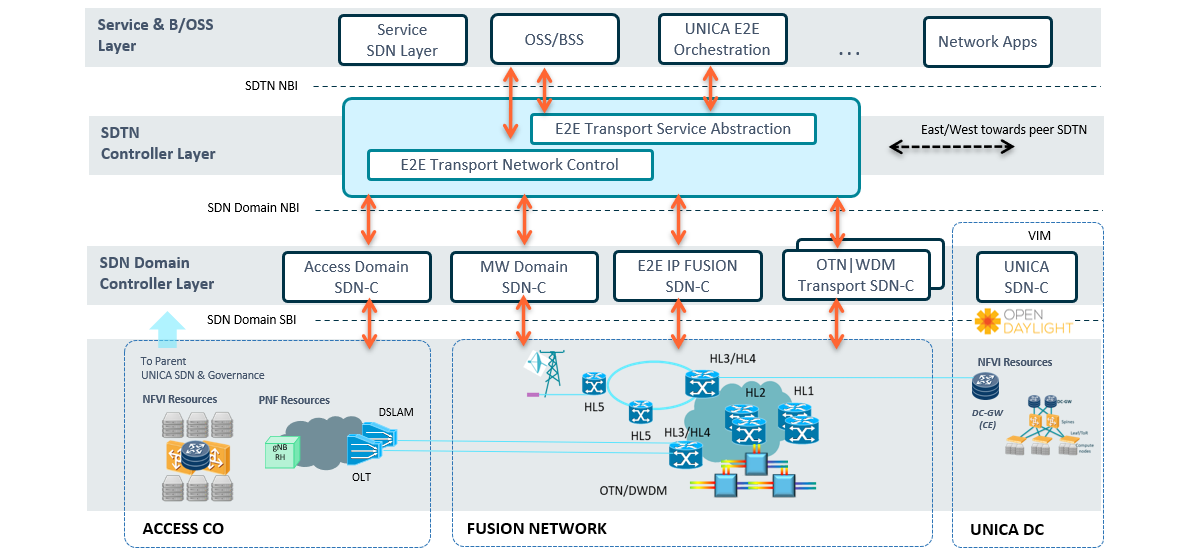
\includegraphics[width=\linewidth]{figs/ifusion_architecture.png}
	\caption{iFUSION architecture}
	\label{FIG:1}
\end{figure*}

The key elements of the SDN iFUSION architecture are the following:

\begin{itemize}
\item \textbf{SDN Domain}: It is a set of network elements under the supervision of the same SDN Controller. There are several possible levels in the decoupling of control and data planes. The preferred level of decoupling in Telefonica depends on the network technology. For example, in the case of MPLS, the network element runs the distributed protocols (e.g. IS-IS TE, RSVP-TE) and the controller only needs to configure it.

\item \textbf{SDN Transport}: It is the whole network controlled by following SDN principles. It is divided into SDN Domains for technology/scalability/administrative principles. A SDN Transport Controller (also referred as SDN Orchestrator), will take care of stitching the different domains/layers/technologies.

\item \textbf{SDN Domain Controller}: This element is in charge of a set of network elements. It has standard southbound interfaces that depend on the technology, but not in the equipment vendor, to communicate with the network elements. It also has a northbound interface to communicate with the SDN Orchestrator and the OSS.

\item \textbf{Software Defined Transport Network (SDTN) Controller}: In case several SDN Domains are needed, the SDN Transport Controller is in charge of providing services through several domains. 

\item \textbf{Southbound Interface}: It is the interface, based on a standard, between the SDN Domain Controller and the Network Element. Not only the communication protocol needs to be standard, but also the data model used.

\item \textbf{Northbound Interface}: If is the interface, based on a standard, between the SDN Domain Controller and the OSSs and SDN Transport.

\item \textbf{Service SDN controller}: An additional SDN layer that takes into account services might be needed. 
\end{itemize}

The iFUSION architecture is designed as a hierarchical model where each network segment is controlled by a dedicated SDN Domain controller. The transport network, due to its wide scope and complexity, is divided in three main technology domains: \hyperref[section:ip]{IP} and \hyperref[section:dwdm]{Optical} for transmission and a Software Defined Transport Network \hyperref[section:sdtn]{SDTN} controller.

The Software Defined Transport Network (SDTN) Controller is responsible to orchestrate the respective SDN Domain controllers within the transport segment (IP, Optical and MW) through the Domain Controllers\'NBI, providing an end-to-end transport network vision. The SDTN Controller aggregates demands from the management and services layer exposing a unified NBI which should provide resource configuration abstraction and technology agnostic service definition. 

The SDTN entails the following functions: 
\begin{enumerate}
    \item End-to-end service binding and mapping.
    \item End-to-end Transport Service Abstraction.
    \item End-to-end resource/topology discovery and composition.
    \item End-to-end resource visualization.
\end{enumerate}

The SDN Domain controllers, on the other hand, are in charge of all the devices in the domain. Each SDN Domain controller unifies the device configuration interface and provides vendor-agnostic network configuration, monitoring and resource discovery. Besides, the Domain Controller exposes high-level network services abstraction to OSS and BSS layers through its North Bound Interface (NBI). Therefore, the abstraction of device specific configuration from network service definition is one of the main features that the SDN controller implements. Moreover, the SDN Domain Controllers entail the function of Path Computation Element to manage and optimize traffic engineering in the domain.

\subsection {IP domain}
\label{section:ip}
IP networks are deployed following a hierarchical model, mixing equipment from different vendors. The IP boxes are interoperable at data plane level and control plane level (e.g. routing protocols such as IS-IS, OSPF or BGP). Due to scalability reasons, the IP networks are typically subdivided in IP domains, so the routing and control protocols are confined to their administrative domain.

The foreseen SDN solution for IP segment is based on a single, multi-vendor IP SDN Domain Controller in charge of configuring the IP network elements, as shown in \cref{FIG:2}.

\begin{figure*}
	\centering
		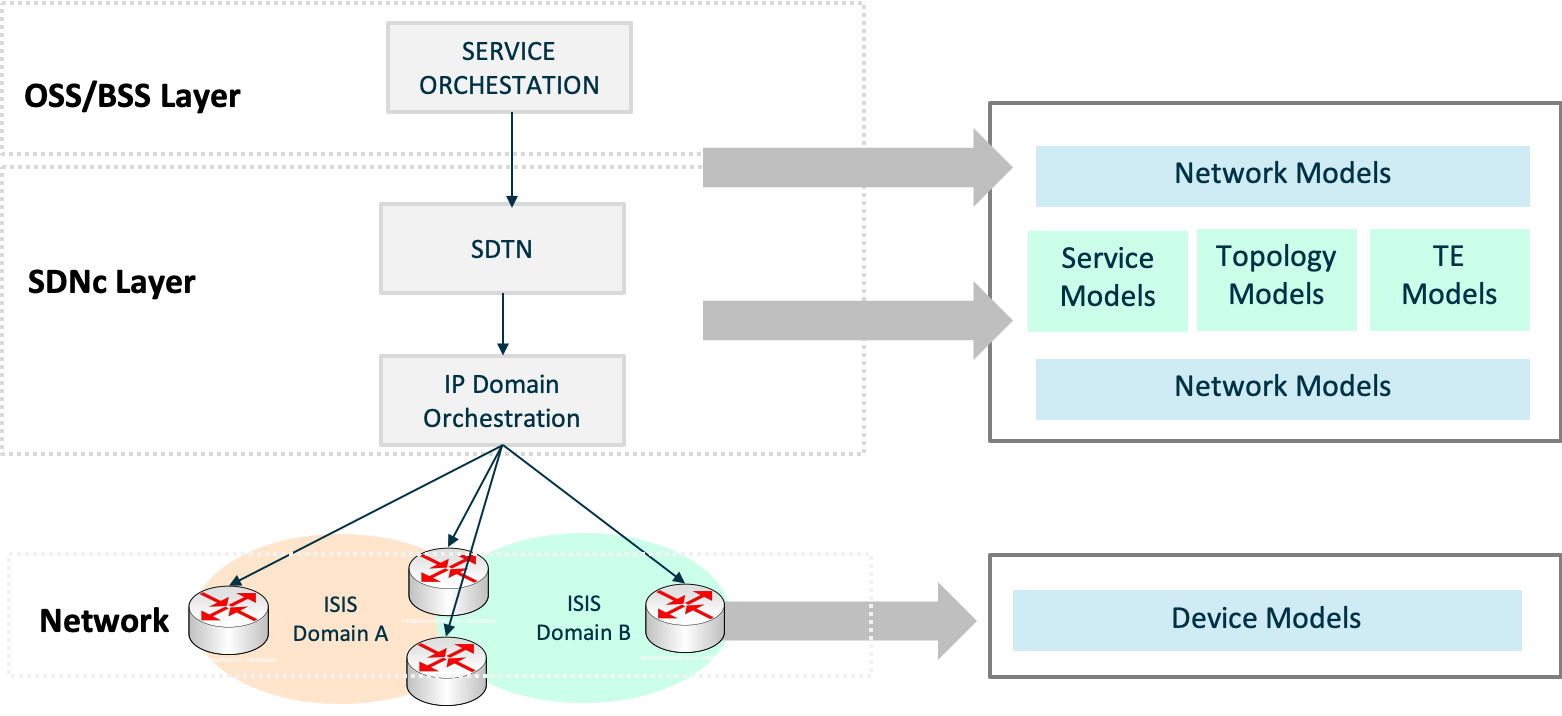
\includegraphics[scale=0.5]{figs/ifusion_multidomain_2.png}
	\caption{Single multi-vendor IP SDN Domain Controller deployment}
	\label{FIG:2}
\end{figure*}

The target SBI for vendor agnostic device configuration shall be compliant with NETCONF standard protocol. The  set of device configuration data models (SBI) are the ones defined in OpenConfig.

The IP SDN Domain controller shall perform Traffic Engineering and Path Computation tasks. With that purpose, some standard and mature control protocols such PCEP and BGP-LS for MPLS networks, shall be implemented to complete the definition of the SBI. As a result,  is expected that the IP SDN controller will assume the control/management of:
\begin{itemize}
\item Device configuration of interfaces (VLANs) and routing protocols (BGP, ISIS…)
\item Traffic Engineering of MPLS tunnels (LSPs). 
\item Overlay networks services (L2/L3 VPNs) device configuration (VRFs,\dots)
\end{itemize}

The IP SDN Domain controller will be the main entry point to the network elements, to avoid overloading the elements and providing a coherent view. The NBI of the controller will also be based on standard models defined in YANG and implemented on RESTCONF with JSON encoding. The NBI shall provide to higher entities within the SDN hierarchy:
\begin{itemize}
\item Device inventory information.
\item A layered topology view (L2/L3, MPLS) of its controlled network entities.
\item LSPs provisioning and path computation.
\item Device abstraction for network services towards the SDTN Controller, i.e., for overlay services VPNs (L2, L3)
\item Network state and performance monitoring information of the IP domain. 
\end{itemize}

\subsection{Optical domain}
\label{section:dwdm}
Transport WDM networks from different system vendors are deployed on a regional basis, either for technology redundancy, due to different optical performance requirements (metro vs. long-haul), or simply for commercial reasons. 

Without line-side interoperability of the different WDM transceivers and Reconfigurable Optical Add-Drop Multiplexers (ROADMs), there is not a competitive advantage on a uniform configuration interface of the optical devices, since they cannot neither be mixed in a multi-vendor scenario, due to the fact that both line systems and transceivers must be from the same vendor.

With this in mind, in the short term, Optical SDN controllers are expected to provide network programmability and interoperability towards upper layers (multi-layer) and between vendors (multi-domain, multi-vendor) through the support of standard NBIs (i.e. coordination will be provided by upper layer hierarchical SDN controller). This short term approach will enable the setup and tear down of connections in optical channels (OCh and ODU layers), the discovery the network resources to compose a layered uniform view based on the OTN hierarchy, and the monitoring of the optical network. 

The SDN architecture proposed is compatible with a legacy control scenario where a distributed GMPLS control plane has been already deployed. GMPLS control plane can be centrally managed by a SDN domain controller by well-know and mature control protocols, such as PCEP, OSPF and/or BGP-LS already supported in GMPLS devices, beneficing the gradual introduction of SDN. However, current NMS solutions shall evolve to, or co-exist with, the SDN Controller model, enabling network programmability through its NBIs while keeping the current offered features for network creation, resources discovery and monitoring and service creation for L0/L1 layers. Standardization efforts targeting the definition of standard NBIs that can facilitate multi-vendor interoperability (by maintaining administrative domains for each vendor) such as ONF Transport API (T-API) \cite{lopez2016transport} and IETF models \cite{wu2017service} are the more promising definitions to implement such capabilities by abstracting the specific configuration of current distributed control planes embedded in Automatic Switched Optical Network (ASON) architectures. 
iFUSION relays on ONF Transport API 2.0 as as the reference NBI for the SDN implementation in the optical transport segment, having been experimented in several proof of concepts \cite{mayoral2016first,mayoral2017control,bravalheri2019vnf}. 

In the medium and long term, the direct programmability of the components can have interest in Point-To-Point, Metro and Regional scenarios, where disaggregation of optical transceivers and line side components can play an important role. In this line, OpenROADM \cite{oda2016learning,kundrat2019opening} and OpenConfig \cite{shaikhopenconfig} projects have already defined device configuration models for transponders and open line systems. Telefonica is approaching this transformation of the optical control in two phases:

\begin{enumerate}
    \item \textbf{Partial disaggregation}: As a medium term objective, where the target is to define a standard interface based on NETCONF/YANG, which allows of the Optical SDN Controller to manage third-party terminal devices (i.e., transponders) that can transmit over the vendor line system.
    
    \item \textbf{Full disaggregation}: The long term objective is the open management of the line system, i.e., the defragmentation of the optical transport network in vendor islands by the adoption of a common standardized interface for open line systems (multi-vendor) to be managed by a single optical SDN Controller.
\end{enumerate}

\subsection{Integration of SDTN in the overall operator’s systems architecture}
\label{section:sdtn}
The SDTN Controller will keep visibility of all the transport network segments. It will expose an abstracted topology view of the network resources and the available set of network services to different clients through its North-Bound APIs.  
One of the main drivers of deploying an SDTN controller is service automation. SDTN will enable it, progressively, facilitating that services and network configurations carried out manually today become automated and available through this abstraction layer.  The level of abstraction can be different according to the needs of the northbound client (e.g. OSS, service orchestrators/SDN controllers, NFV orchestrator, etc.). 

The information exported through the NBI towards OSS and other platforms will cover a number of functional areas. The service’s provisioning, network topology visualization within the Resource Lifecycle Management (RLM) domain will be the first set of functionalities adopted by the SDTN controller; and tested in this paper. Progressively the SDTN will include Performance Management (PM) and Network Planning and Design (NPD), Fault Management (FM) and Resource Inventory Management (RIM) areas. The inclusion of these functional blocks is conditioned to the standardization of the required data models for the SDTN NBI and SDN Domain controllers SBI.

On the SBI of the SDTN, each technology Transport Domain SDN Controller shall expose vendor agnostic network level programmability and resource discovery functionalities. The SDTN Controller SBI is intended, but not limited, to provide access to device’s configuration data, to expose per-OSI layer topology and network inventory information, and to offer active monitoring of device configuration changes and network state data (i.e., traffic statistics). Alarm and device inventory information for FM and RIM respectively, is intended to be managed at the SDN Domain controllers in a first phase, but its exposure through the SDTN will be evaluated too.


\section{Network Programmability}
\label{section:net}

The network management has lagged behind other technologies quite drastically. In more than 20 years, there has not been radical improvements in the device management area. One of the major advances was related to the usage of SSH instead of TELNET for secure implementations. However, scripts based on EXPECT are the most programmatic way to access the devices in the service providers across the globe.

This lack of manageability is often better understood when networking is compared with other technologies. For example, hypervisor managers, wireless controllers, IP PBXs, PowerShell, DevOps tools are part of the continous Integration and continous Development (CI/CD) in cloud providers \cite{mittal2017cloud,demchenko2016zerotouch}. Some of these are tightly coupled from a certain vendor, but others are more loosely aligned to allow for multi-platform management, operations, and agility \cite{edelman2018network}.

To allow the network programmability it is completely necessary to use SDN as the reference for the introduction of network APIs. It must be taken into account that these network APIs are not just related to the service provision automation (provision is a repetitive task and its components can be described in a technological way). The usage of APIs and programmatic interfaces can automate and offer much more than pushing configuration parameters. 

It can be used to cover all the FCAPs (Fault, Configuration, Accounting and Performance) capacities and Network planning tasks:
\begin{itemize}
    \item Network planning tasks if we include APIs to export distributed information such as the RIB, FIB, and TE-Databases.
    \item Used to deploy close-loop decision systems to take actions based on events reported by the devices.
    \item Automatically visualize the network relationships between the IP/MPLS and Optical packet transport domain. Creating a common network view. 
\end{itemize}

\section{Service Models}
\label{section:models}

Due to the network programmability necessities. Protocols and Data models must be selected to allows the interaction between the network controllers and devices. There has been a great interest in using YANG to define these data models. However, this YANG definition may include two groups of models. One set used strictly to attack the devices and the ones used to describe services in a portable and technological way (independent of which network operator uses the model). 
This differentiation between Service and Device Models introduced in early 2018, would allow abstract some information in the control layer. The service models may be used as part of the SDN architecture, describing the data interchanged between the network controllers and between OSS systems and the control Layer \cite{wu2017service}. While the device models described the specific configuration of the network elements. 

Example of service models definitions are described in the following sections: Section \cref{section:IPmodels} for IP and \cref{section:OPTmodels} for Optical.

\subsection{IP Network Models}
\label{section:IPmodels}

This section describes the service models used for the field trial. The IP service models are YANG modules defined to support the creation, deletion and retrieval of \hyperref[section:l3nm]{L3}/ \hyperref[section:l2nm]{L2VPN}. The ones defined to collect the network \hyperref[subsection:IPtopo]{topology} from the IP/MPLS network are also explained. The models described in this section are abstract models that technologically describes the network requirements and are RFCs or working-group-drafts inside the IETF.

\subsubsection{L3NM}
\label{section:l3nm}
The Layer 3 Virtual Private Network (VPN) service defined in RFC 4364 \cite{rosen2006rfc} provides a multipoint, routed service to the customer over an IP/MPLS core. The L3VPNs are widely used to deploy 3G/4G, fixed and enterprise services principally due to the fact that not only several traffic discrimination policies can be applied across the transport network but also because several stitching methodologies can be applied to combine access and transport services. 

Some service models has been defined and standardized until now to support the L3VPN creation. L3SM \cite{rfc8299} is a Customer Service Model that describes the requirements of a L3VPN service based on the customer requirements; The L3SM model keeps some commercial customer parameters as the customer site location.

L3NM \cite{voyer2019internet} is a complementary Network Model of the L2SM. It differs from the L3SM because It is completely network-centric, it is focused on the service provider's internal network configurable parameters more than the customer information. The L3NM can be exposed by network controllers to manage and control the VPN Service configuration in multi-domain scenarios and It contains information of the service provider network such as NE-ID and Interfaces-ID and might include allocated resources such as the Route Targets (RTs) and Route Distinguishers (RDs).

The L3NM model will be used in this field trial as the data model used between the SDTN and the IP SDN Network controllers. The SDTN network controller will include network-specific information in the service request (i.e. transport LSP binding, routing profiles or encryption); and in order to facilitate the multi-domain orchestration, the SDTN will assign some logical resources (such as route targets or route distinguishers) that must be synchronized between domains. \Cref{FIG:l3nm} shows the structure of the YANG data model, where the main container (VPN Service) is used to group the information of the VPN-Node (VRFs) and the VPN-Network Accesses (Interfaces).

\begin{figure*}
	\centering
		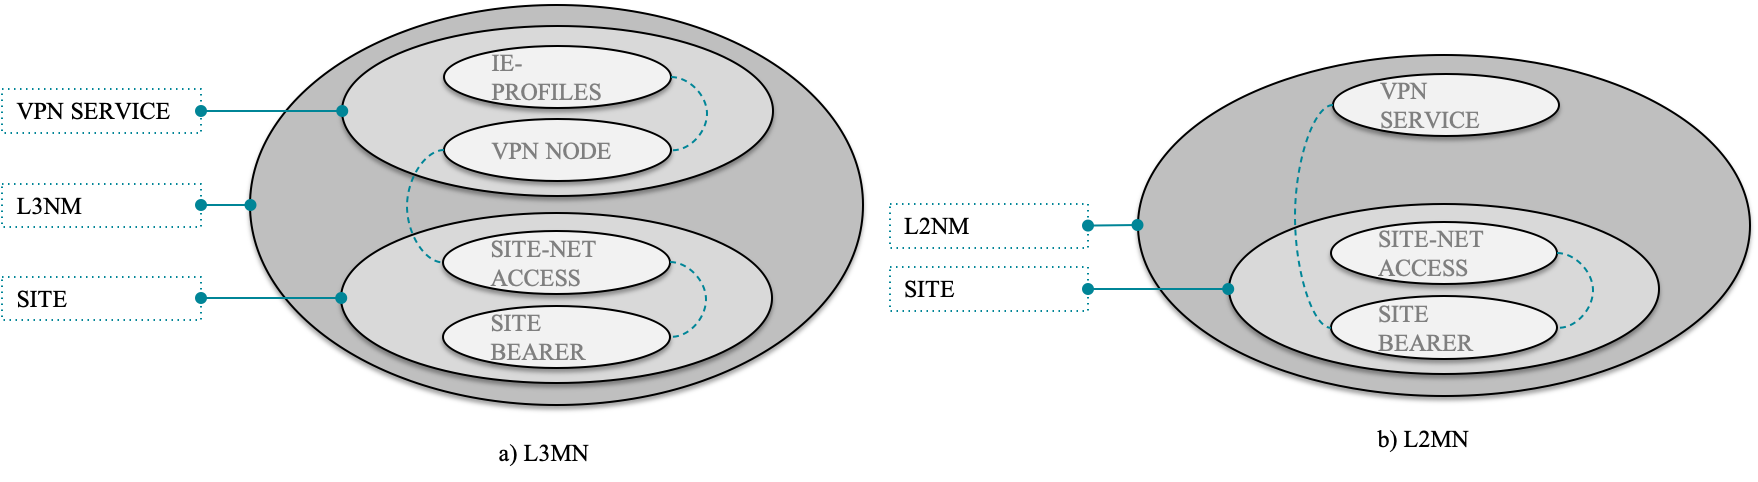
\includegraphics[scale=0.35]{figs/L3NM_L2NM.png}
	\caption{L2NM and L3 Data models structure}
	\label{FIG:l3nm} 
\end{figure*}

\subsubsection{L2SM}
\label{section:l2nm}

L2 services belongs to the class of IP virtual leased line services (VLLs) or virtual private LAN services (VPLS)\cite{andersson2006framework}, which are a fundamental part of the service portfolio offered by SPs. 
VLLs and VPLS can be generally described as point-to-point or point-to-multipoint solutions, respectively. In the same way as the L3SM is the service model proposed for the L3VPNs is there already an equivalent for the L2 services. The model is named L2SM \cite{wen2018yang}. 

As the L3, the L2SM is a customer centric model. It has two main containers the VPN Service and the site depicted in the rigth side of \cref{FIG:l3nm}. The service container has all the technological parameters of the services that is going to be deployed, for example: service type (i.e. bgp-vpls, pw3, ldp-vpls, \dots) or service topology (i.e. p2p, p2mp). The site container has all the customer information, including the customer-location, and the connectivity parameters between the CE and the PE. 

This model miss some specific network configuration, that need to be stored or derived by the network controller to deploy the final configuration on the network devices. An additional work to complement this model can be proposed for futures implementations.  

\subsubsection{Network Topology}
\label{subsection:IPtopo}

The proposed control architecture relies on providing different levels of abstraction for each control layer. Therefore, the needs in terms of topology and knowledge of the service provider network differ among components. 

Network topology is an abstract representation of the physical nodes, links and network interconnections. It is crucial to get and graphically represent network information, such as:
\begin{itemize}
    \item Structure (Connectivity and Paths)
    \item Performance (Available bandwidth per link)
    \item Availability of physical and logical resources
\end{itemize}

Currently, the topology representations are limited to the scope of each of the network vendors i.e Each NMS has its particular/proprietary network view. Sometimes Dummy devices from a third party can be included to simulate the interconnection of the networks. However, nowadays obtain a unified view of the entire IP network is not possible.

However, as part of the I2RS working group on the IETF a common base model for an initial network topology representation has been defined. The model includes: Nodes and Links. As a complementary work, several augmentations has been done to cover the L2, L3 and TE functionalities.

In this implementation, the topology models used to retieve the IP network are: 
\begin{itemize}
\item IETF Network (RFC8345): Includes the Network, Node and Link concepts \cite{clemm2018yang}.
\item IETF Network Topology (RFC8346): Includes Termination-Points inside the Nodes and IP specific parameters such as addressing information \cite{varga2018internet}.
\end{itemize}

\subsection{Optical Network Model}
\label{section:OPTmodels}

In this section the reference standard model use for the control/management of networks based on WDM/OTN technologies is described. The proposed solution for the Northbound Interface of Optical Domain SDN-C is based on ONF T-API information models and the RESTCONF protocol. Please note, that in this transport domain, the same solution (T-API + RESTCONF) is also proposed to be the NBI of the hierarchical SDTN Controller towards Service B/OSS layer.

\subsubsection{Provisioning}

\begin{figure*}
	\centering
		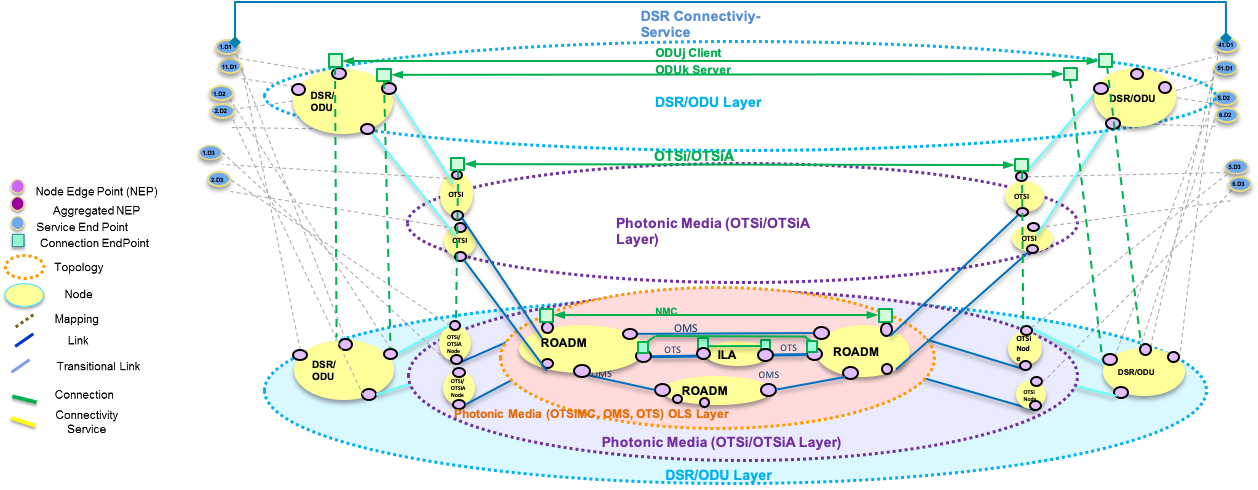
\includegraphics[scale=0.8]{figs/ONF-T-API.png}
	\caption{Multi-layer topology and connectivity models based on ONF T-API}
	\label{FIG:ONF-T-API}
\end{figure*}

The connectivity provisioning into the WDM/OTN optical layers is strictly related with the model proposed. \Cref{FIG:ONF-T-API} represents the optical network topology arrangement proposed in the previous figure and the multi-layer hierarchical connectivity modelling which is being detailed in this section.

The connectivity model introduces to central concepts. On one hand, the tapi-connectivity:connectivity-service  object models "intended" solicited by the T-API client layer, to be deployed into the network. On the other hand, the tapi-connectivity:connection objects represents the actual adjacencies between logical interfaces created by configuring the network, in brief the connectivity configurations in the network. 

The network model is multi-layer so it is needed to establish multi-layer relationships into the model. These relationships are construct by the relationship between Logical Termination Points (LTPs) which in T-API are modelled as two different objects: the Node-Edge-Points (NEPs) which represents the resources available at a give layer LTP to provide connections, and the \textbf{Connection-End-Points (CEPs)} which consumes part of all of the NEPs exposed resources to create the connections between different points of the network. In our proposed reference implementation, we distinguish between two different level of connections:

\begin{itemize}
    \item \textbf{Cross-Connections (XC)}: defined as a connection between Connection-End-Points of the same layer within a Forwarding-Domain (represented as a\\ \texttt{tapi-topology:node} object). 
    \item \textbf{Top Connections}: are defined as end-to-end connections between CEPs within the same layer which may span multiple Forwarding-Domains. Top connections are composed by zero or more XCs which belong to the same layer of the Top Connection.
\end{itemize}

Then, the multi-layer relationships are construct by stacking CEPs over NEPs and providing the upper layer resources representations by the dynamic creation of new NEPs, e.g., an OTSi connection, when created and operational, it provides the ODU upper layer resources in the form of NEPs which in turn can be consumed to create ODU connections which will provide the DSR layer resources.

\subsubsection{Topology}
\label{subsection:OPTopo}

The topology model should provide the explicit multi-layer topology representation of the L2-L0 network including OTS, OMS, MC, OTSIMC, OTSi/OTSiA, ODU, DSR layers. The network logical abstraction collapses all network layers (DSR, ODU, OTSi/OTSiA and Photonic Media (OTSiMC, MC, OMS, OTS)) which are represented explicitly into a single topology (T0 – Multi-layer topology), modelled as a \texttt{tapi-topology:topology} object within the: \\
\texttt{tapi-topology:topology-context/... \\
... tapi-topology:nw-topology-service} and \\ \texttt{tapi-topology:topology-context/topology}. 

The T0 – Multi-layer topology MUST include:

\paragraph{DSR/ODU Layers:}
DSR/ODU forwarding domains represented as multi-layer and multi-rate \texttt{tapi-topology:node}, allowing the representation of the internal mapping between DSR and ODU NEPs (multi-layer) and the multiplexing/de-multiplexing across different ODU rates (multi-rate). 

The DSR/ODU layer network MUST be represented explicitly at the lowest partitioning level, i.e., each DSR/ODU forwarding domain MUST be represented as a single tapi-topology:node. The following network components included within the category of ODU forwarding domain are:

\begin{itemize}
    \item Transponders.
    \item Muxponders.
    \item OTN switching nodes connecting client and line boards.
\end{itemize}

\paragraph{OTSi/Photonic Media layers:}
The OTSi layer represents the optical side of the optical terminals (transponders/muxponders). This layer consists of nodes representing the mapping and multiplexing of OTSi signals. It consists of nodes including OTSi client endpoints representing the Trail Termination Points (TTPs) of the OTSi connections and OTSi/OMS endpoints representing the physical connectivity with ROADM/FOADM add/drop ports.

DSR/ODU and OTSi layers may be collapsed into a single multi-layer node or split into two logical nodes representations by using the Transitional links concept to represent the potential layer transitions between ODU and OTSi.

\paragraph{Photonic-Media layer:}
The Photonic-Media layer models the Optical Line Protection  (OLP) components, the Reconfigurable/Fixed Optical Add Drop Multiplexers (ROADM/FOADM) and In-Line Amplifiers (ILAs) network elements. Moreover, all the lowest photonic connectivity is represented as PHOTONIC\_MEDIA \texttt{tapi-topology:link} objects collapsing OTS/OMS layers and allowing placing specific monitoring OAM functions of these layers. These forwarding domains SHALL expose the capability of create Media Channel connection and connectivity services between its endpoints.

\begin{figure}
	\centering
		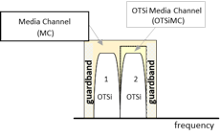
\includegraphics[scale=0.75]{figs/Media_channel.png}
	\caption{Media-channel entities relationship}
	\label{FIG:Media_channel}
\end{figure}

Moreover, the Media Channel layer the available resources for the reservation of  spectrum resources for a given OTSi channel. The concatenated reserved portion of the along a route is represented as a Media-Channel (MC) construct, and by the OTSiMC construct which represents the actual portion of the spectrum occupied by the signal (MC spectrum must be wider than the OTSiMC). These modelling concepts are critical for the realization of the Open Line System concept introduced by the partially disaggregation of the optical networks. See \cref{FIG:Media_channel} graphical representation for more clarity.


\subsection{End-to-end Use Cases Definition}
The two end-to-end uses cases defined for testing in this work are described in the next subsections:

\subsubsection{Multi-domain IP L3VPN provisioning}
\label{section:muli-l3nm}

As described previously in the \cref{section:l3nm} the L3VPNs services are not exclusive of single domain implementation. Multi-domain IP L3VPN is a common requirement in the service providers. The reality of the brownfield scenarios is multiple-AS, multiple-IGPs, or multiple-vendor segmentations. Despite this, the service provision process may require a set of interactions with more than one IP SDN Controller. 

The scope of this work includes two domains within the same network. Each domain is controlled by an independent SDN Controller. Each controller has implemented the IETF L3NM model described in subsection \cref{section:l3nm}. We have proved the SDTN as a network orchestrator to delegate the required provision parameters to each controller and expose an unified view of it.

\begin{figure}
	\centering
		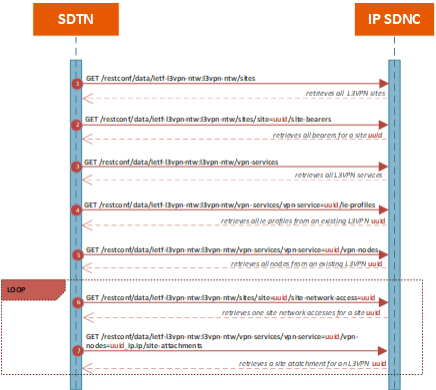
\includegraphics[width=\linewidth]{figs/l3vpn_workflow.png}
	\caption{Messages Interchange for IP multi-domain L3VPN service creation.}
	\label{FIG:l3vpn_workflow}
\end{figure}

For this specific use case, the parameters and request will have the following four steps per each domain. \cref{FIG:l3vpn_workflow} depicts the corresponding workflow where the following steps are needed to provision the multi-domain service:
\begin{enumerate}
    \item Create Site (VPN.L3.Site.Add)
    \item Create Bearer (VPN.L3.Bearer.Add)
    \item Create VPN (VPN.L3.Add)
    \item Create Access (VPN.L3.Access.Add)
\end{enumerate}

%\begin{figure}
%	\centering
%		\includegraphics[width=\linewidth]{figs/multidomain_service_provisioning%_workflow.png}
%	\caption{Workflow for multi-domain service provisioning SDTN-SDN-C}
%	\label{FIG:multidomain_service_provisioning_workflow}
%\end{figure}

\subsubsection{Multi-layer Topology}

The multi-layer topology use case is based on the data provided by all the \hyperref[subsection:IPtopo]{IP} and \hyperref[subsection:OPTopo]{Optical WDM/OTN} SDN-Controllers. The scope of it, includes the composition of multiple sources and data-formats (i.e IETF context for IP or T-API context for Optical) to create a common view of the network. The models used to create the multi-layer topology were:
\begin{itemize}
    \item For the optical domain representation: Topology and Connectivity Service modules. Those models provides information for layers from L0 to L2.
    \item For the IP/MPLS domain representation:  The \texttt{ietf-network:networks} is the basic to expose the network model(nodes and IP Links), and the \texttt{.../node/nt:termination-point}
    were used to expose the Terminations-points (Ports) of a specific node.
\end{itemize}
    
Additionally, a correlation parameter were defined to to join the IP and Optical layers. This parameter is the \texttt{plug-id}. This additional definition were needed becasuse there is no a dynamic protocol or common element between the ONF/IETF standards that would allow their correlation. The \texttt{plug-id} parameters were added in the IETF termination points and in the TAPI Connectivity Services. 

It os necessary to remark in the T-API model side the Plug-id parameter is a "String" and in the IETF side is "Binary", therefore the SDTN controller MUST have the ability to traduce the “Binary” value to “String” or vice versa, to be able to make the match in the correlation process considered to be standardized.

To fill the Plug-id attribute automatically between the layers, it is required that the SDTN performs a process based on meta-heuristic algorithms. In which, the performance data at termination-points level both in the IP and in the Optical layers are correlated. Clock \& Time must be perfectly synchronized between the Tx/Rx points, bidirectionally. Meta-heuristics must include the geo-location parameter of the nodes as input. However, the design of this process is currently under study and is based on real-time information that can be delivered by the telemetry engines.

\begin{figure}
	\centering
		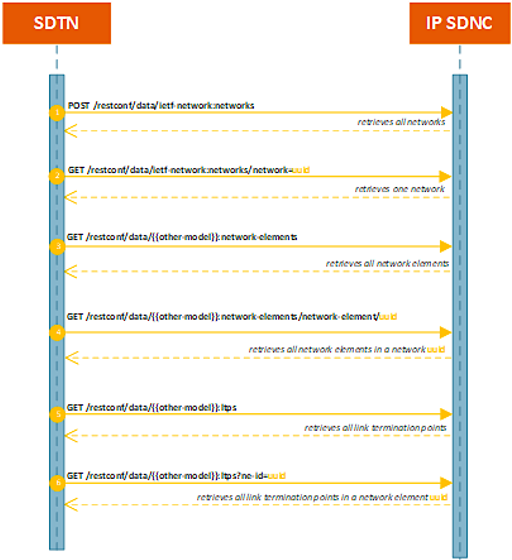
\includegraphics[width=\linewidth]{figs/ip_topology_workflow_2.png}
	\caption{Message Interchange for IP Topology Discovery}
	\label{FIG:ip_topology_workflow}
\end{figure}

In this work, the construction of the multi-layer topology, the SDTN performed the task of value correlation between layers, using manually filled "plug-id" attributes in IP and Optical layers. The process proposed is depicted as workflow in \cref{FIG:ip_topology_workflow}.

%\begin{figure}
%	\centering
%		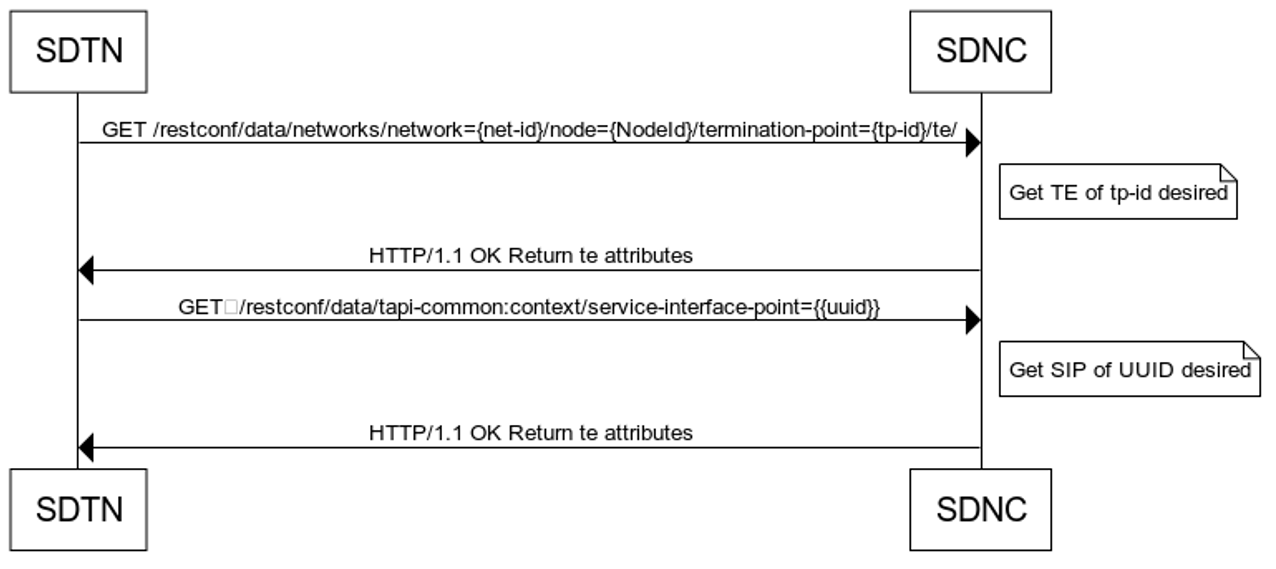
\includegraphics[width=\linewidth]{figs/topology_workflow.png}
%	\caption{Workflow for multi-layer topology SDTN-SDN-C}
%	\label{FIG:topology_workflow}
%\end{figure}

\begin{figure*}
	\centering
		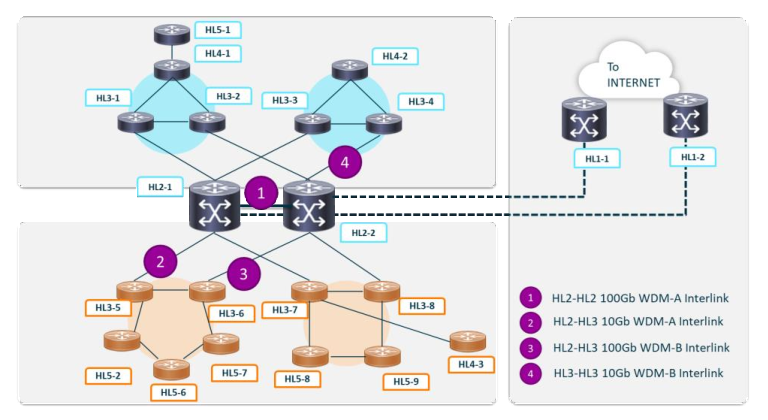
\includegraphics[scale=1]{figs/field_trial_environment_ip.pdf}
	\caption{Network Plane of the Field Trial Environment for IP/MPLS Testing and Evaluation}
	\label{FIG:field_trial_ip}
\end{figure*}

\begin{figure*}
	\centering
		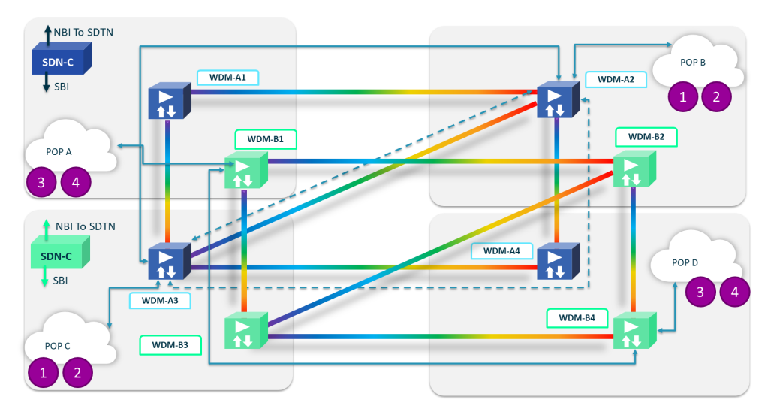
\includegraphics[scale=1]{figs/field_trial_environment_optical.pdf}
	\caption{Network Plane of the Field Trial Environment for Optical/WDM Testing and Evaluation}
	\label{FIG:field_trial_optical}
\end{figure*}

\section{Field Trial Environment for iFusion SDTN Demonstration}
\label{section:trial}

A field trial environment to demonstrate, test and evaluate the end-to-end multi-domain cases and the SDN-based iFusion Architecture were developed. It has two main layers: Fistly, a \hyperref[sec:contol_lay]{Control Layer} is comprised of two SDN IP Domain Controllers for a multivendor IP/MPLS network using as underlying WDM infrastructure and working in parallel with two SDN Optical Domain Controllers. On top of that, a multilayer multidomain SDTN Controller is orchestrating the uses cases. Secondly, the \hyperref[sec:net_lay]{Network Layer} is comprised of a Metropolitan WDM Network with nx100Gb Lambda capacity providing interlink capabilities for a multidomain IP/MPLS network following a hierarchical architecture that we denominate from HL1 (Hierarchical Layer No. 1) to HL5. We detail each of the layers in the next subsections. 

\subsection{Control Layer}
\label{sec:contol_lay}
A hierarchical SDTN architecture is built upon the reference design guidelines described in \cref{section:arq}. The kay elements of the control layer was:
\begin{itemize}
    \item Infinera Trascend Maestro, acting as SDTN controller.
    \item 2 x IP Domain Controllers one for each cluster.
    \item 2 x Optical Domain Controllers one for each cluster.
\end{itemize}

From the IP control perspective, SDN-Cs communicate with NEs via NETCONF/YANG and RESTCONF/YANG with SDTN.  In other hand, from the Optical perspective, SDN-Cs follow a similar integration. At SBI, OpenROADM + OPenConfig models are used on top of NETconf/YANG protocol. At NBI, a T-API implementation is used.  

\subsection{Network Layer}
\label{sec:net_lay}
We use a scale representation in terms of quantity of equipment but a full network field trial with all the hierarchical layers that compose a Service Provider real deployment. In our notation and architecture the IP/MPLS-base network is comprised of five (5) layer with the following responsibilities: 
\begin{itemize}
    \item HL1: Core P/PE-Routers acting as Toll Gates for interconnection the Service Provider to the International Exit and using eBGP logical structure for publishing public IPv4/IPv6 prefixes to IP gates from and to a Tier-1/2 international Internet provider.
    \item HL2: Core P-Router responsible for the transportation of traffic between main cities and metropolitan areas sending/receiving traffic to HL1 interconnections from/to the International Internet.
    \item HL3: PE-Routers responsible for the aggregation and conglomeration of traffic from metropolitan and regional areas coming from network clusters and rings covering main and secondary cities for both fixed and mobile services.
    \item HL4: PE-Routers able to collect traffic from fixed access networks (DSLAM/CMTS/OLT) in metropolitan areas and high capacity corporate services. And to collect traffic from mobile access networks coming from HL5 (former cell-site routers) for all generations 2G/3G/4G, 4.5G and new 5G in the near future.
    \item HL5: Provides connectivity access to corporations, enterprises, small businesses and mobile terminal nodes (BTS, NodeB, eNodeB) in remote areas. Formerly known as cell site routers in Mobile Service Providers, but now evolved and converged to serve multiple fixed plus mobile segments.     
\end{itemize}

The IP/MPLS network was build using seamless MPLS option-C. The Networks is organised by clusters and rings within. Each IP cluster groups devices of a specific vendor. As a seamless MPLS the underlay signalling requires that every origin PE-Routers (HL4) from a cluster, can establish an end-to-end LSP to the destination PE-Router(HL4) even if the destionation belongs to a different cluster. 

Thus the HL3 routers from each region establish an eBGP session against the Core-Routers (HL2). This session exports the Router-ID plus Label information of all the routers in the region using BGP-LU \cite{rfc8277}. Additionally, there is another eBGP session between the HL3 of the region and the core Router-Reflectors to export the VPNv4 routes from each VPN service. This eBGP session requires a mandatory a Next-Hop-Unchanged configuration to avoid network loops or misconfigured paths. All of this control plane setup allows the creation of an end-to-end LSP from the access layer to the platforms without changing the configuration during the service provisioning.

Additionally, to deploy any of this service the network has to fulfill the following basic requirements established between origin and destination:
\begin{itemize}
    \item PEs connectivity based on IGP Router-ID/Loopback reachability.
    \item Label switching protocol enabled. MPLS and Labelling mechanism LDP, RVSP, other. 
    \item MP-BGP sessions between the PEs (address-family vpnv4/6, ipv4/6).
    \item Virtual Routing network instance. 
\end{itemize}

Four (4) IP/MPLS-based network links are transported by a two-vendor WDM underlying infrastructure. \Cref{FIG:field_trial_ip} depicts in purple the four interlinks 2x100Gb and 2x10Gb.  

Regarding the optical transport infrastructure, we have built a dual-plane independent metropolitan WDM networks. Comprised of a ring of (4) four nodes each with nx100Gb and nx10Gb lambda capacity. \Cref{FIG:field_trial_ip} illustrates the optical WDM part of the field trial enviroment.


\section{Test Results}
\label{section:results}

Test results for the Hierarchical SDTN Controller integration with the third-party vendor SDN-C controllers in the Optical and IP domains are presented in this section. Two types of tests have been done in order to demonstrate orchestration functionalities in the multi-layer/multi-domain/multi-vendor network environment, previously described: a) One of them involves the use of Postman as an emulated OSS tool, to send API-based queries towards each of the SDN-Cs, as well as to retrieve the network information as exposed by the domain controllers; b) the second type of test consisted on using Transcend Maestro Web Portal GUI for a user-friendly visualization of the use case deployment.

\Cref{TAB:tested_use_cases} shows the uses cases tested on the network scenario, these have been classified into three main categories: Topology discovery, IP service provisioning and Optical service provisioning. A general overview and the results obtained for each of them are approached individually in further sub-sections of this chapter. Regarding the single-domain use cases, results are shown independently for each vendor and for each network domain in particular.

\begin{table*}
	\caption{List of Multi-Layer Multi-Domain Tested Use Cases}
	\centering
		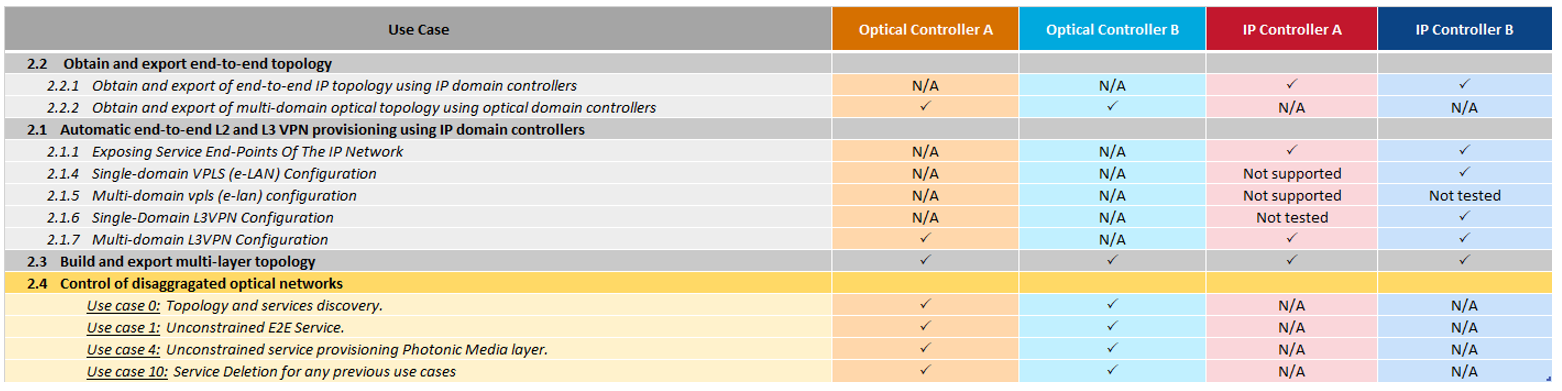
\includegraphics[scale=0.5]{figs/tested_use_cases.png}
	\label{TAB:tested_use_cases}
\end{table*}

\subsection{Multi-layer Topology Discovery \& Visualization}
Obtaining the end-to-end multi-layer and multi-domain topology via automatic network discovery is considered the starting point towards the deployment of the SDTN multi-layer solution in the network scenario described in Section 5. The first and most important step is for SDTN to discover all the network elements of the different domains by using the APIs provided by each of the IP and Optical Controllers. 

\begin{figure}
	\centering
		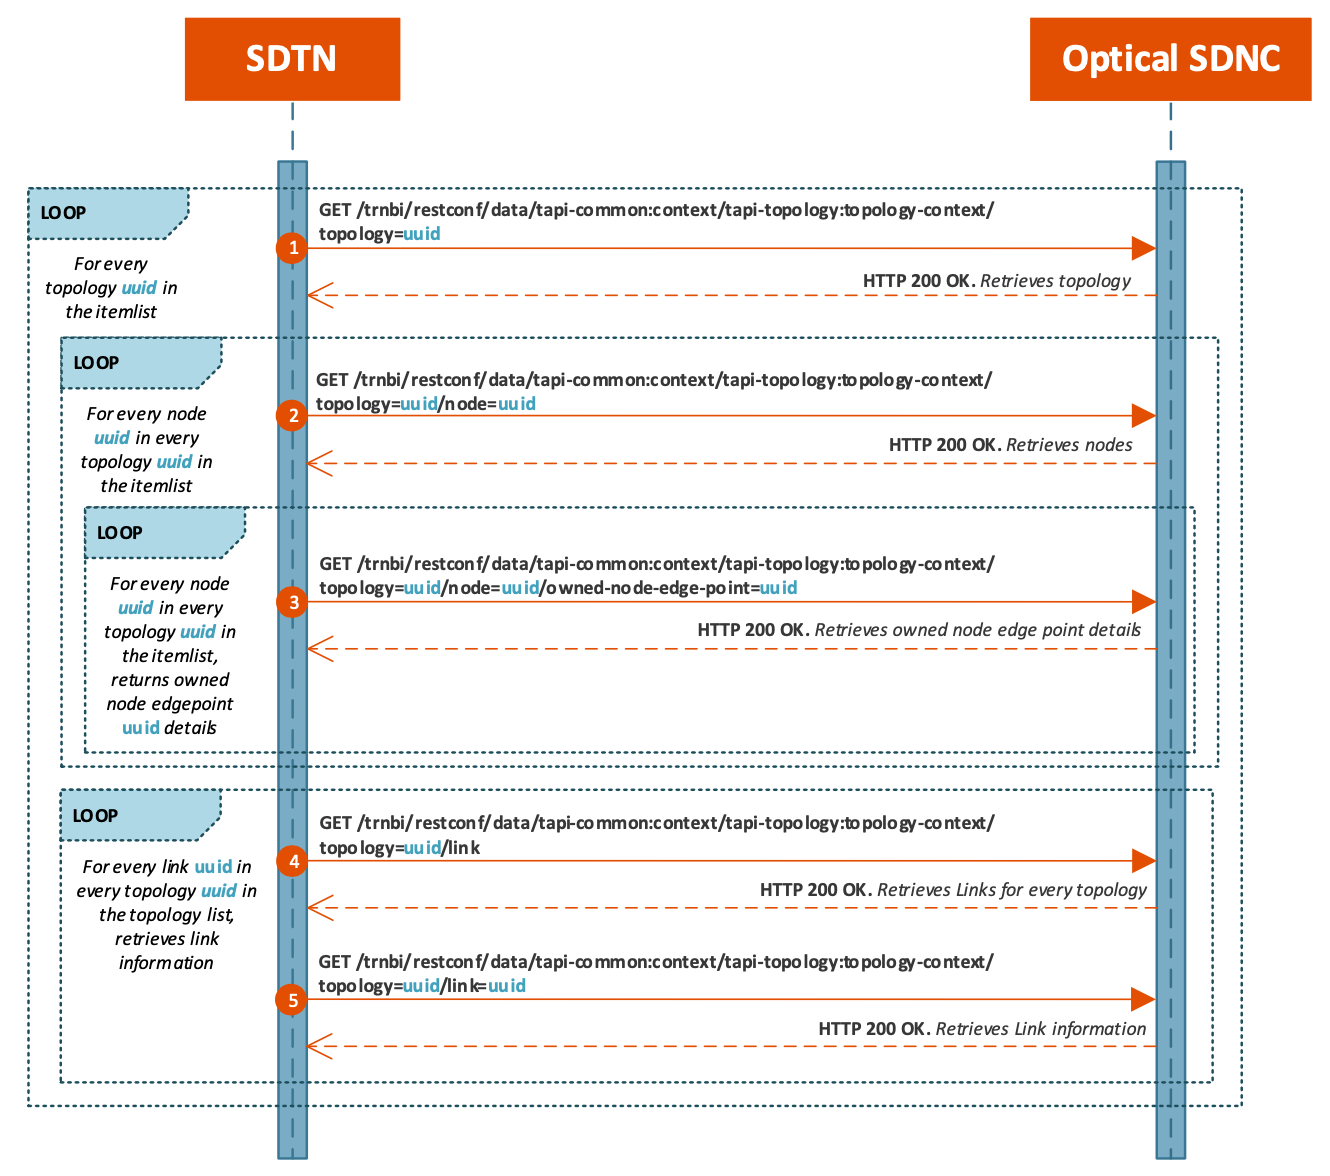
\includegraphics[width=\linewidth]{figs/optical_topology_workflow_2.png}
	\caption{Messages Interchanged for Optical Topology Discovery between the SDTN and Optical SDN Controller}
	\label{FIG:optical_topology_workflow}
\end{figure}

The following steps take part of the end-to-end network discovery procedure:
\begin{enumerate}
    \item \textit{Enabling Network Adapters}: The network for each domain was discovered from the domain controllers individually by using Domain Adapters; each adapter uses the API provided by the Domain Controller to retrieve data such as nodes, inventories, termination points, links and services within it.
    \item \textit{Data Model Mapping}: The information model used in the Domain Controller's API is mapped into the SDTN model in order to harmonize the data across all domains, providing both a per-layer view within the inter-layer links and client-server relationships, thus resulting in a complete multi-layer view of the network and its services.
    \item \textit{Inter-domain links discovery}: End-to-end view of the whole network topology is formed by discovering the inter-domain links. Those interconnect the different vendors into a whole end-to-end multi-layer and multi-domain topology. There are many different mechanisms\footnote{TTI or plug-id for L0/L1, LLDP for L2, IP address based discovery for L3, among others such as alarm/statistics correlation with or without test data/circuits, inter-domain links simulation if no automatic mechanism is available} 
    to achieve this purpose, such as TTI for OTU links, IP addresses for IP links etc. If all the data required for full inter-domain and inter-layer link discovery is not reported by the third-party controllers, external data can be fed in via the SDTN NBI. 
\end{enumerate}

Starting with the Optical Domain, a set of T-API version 2.1 queries were sent in order to build the topology by extracting the list of networks as well as topology details such as nodes, links, connections and service-interface-points available. The query exchange process between is shown in the UML diagram depicted in \cref{FIG:optical_topology_workflow}.  

Regarding the IP Domain, to obtain the whole network topology, a query to the controller’s NBI to retrieve the network topologies available for all layers is sent; from here on, the client must perform per-layer queries to get more detailed information such as nodes, termination points of nodes, links, etc. \Cref{FIG:ip_topology_workflow} displays the RESTCONF based queries in UML format for the topology retrieval in the IP Domain. 

At this point, no interdomain links were retrieved since there is no automatic mechanism supported on the domain controllers to expose information such as TTI (on the Optical Domain), LLDP (on the IP Domain) or Plug-id (for both domains); therefore Plug-id based link discovery was simulated by adding user defined Plug-Id values to each port or at least to each domain edge port manually with the use of python scripting. The inputted plug-id data was automatically detected by the SDTN and the inter-domain links between ports with matching plug-ids were created, resulting in a complete multi-layer/multi-domain end-to-end topology as seen from the SDTN GUI.

The number of discovered elements within the end-to-end network topology is summarized in \cref{TAB:discovered_elements}, for the optical domains in particular, the number of nodes for each topology correlates to the different layers such as:
PHOTONIC\_MEDIA LAYER, DSR LAYER and ODU LAYER as defined in the YANG data model for T-API 2.1, hence the reason why there are more nodes retrieved other than those which are physically implemented in the testbed scenario. Additionally, the service interface points (SIPs) discovered for the Optical Domain are exposed in the Controllers NBI, making it easier for the SDTN to access these parameters and using them for future service provisioning. 

In the IP domain however, given the different models implemented on the IP Controllers, the service end-points were not exposed to the SDTN SBI, reason why the interfaces and ports were needed to be configured manually via python scripting, being this a drawback when it comes to working with models which don’t follow a fully standardized model.

\begin{table*}[]
\caption{Discovered Network Elements for the Topology Visualization}
\begin{adjustbox}{width=1\textwidth}
\small
\begin{tabular}{lllll}
\hline
{\color[HTML]{000000} } &
  {\color[HTML]{000000} Optical Controller A} &
  {\color[HTML]{000000} Optical Controller B} &
  {\color[HTML]{000000} \begin{tabular}[c]{@{}l@{}}IP Controller A\end{tabular}} &
  {\color[HTML]{000000} IP Controller B} \\ \hline
{\color[HTML]{000000} \begin{tabular}[c]{@{}l@{}}Discovered nodes \\    (physical and logical)\end{tabular}} &
  {\color[HTML]{000000} 17} &
  {\color[HTML]{000000} } &
  {\color[HTML]{000000} 11} &
  {\color[HTML]{000000} 13} \\
{\color[HTML]{000000} \begin{tabular}[c]{@{}l@{}}Discovered links\\    (physical and logical)\end{tabular}} &
  {\color[HTML]{000000} 18} &
  {\color[HTML]{000000} } &
  {\color[HTML]{000000} 13} &
  {\color[HTML]{000000} 15} \\
{\color[HTML]{000000} Discovered service-end-points\footnote{The amount of end-points discovered for the domains not only comprehend those available for service provisioning, but all those available in the network }} &
  {\color[HTML]{000000} 97} &
  {\color[HTML]{000000} 90} &
  {\color[HTML]{000000} Not automatically discovered} &
  {\color[HTML]{000000} Not automatically discovered} \\
\rowcolor[HTML]{EFEFEF} 
{\color[HTML]{000000} Intra-domain IP links} &
  \multicolumn{4}{c}{\cellcolor[HTML]{EFEFEF}{\color[HTML]{000000} 2}} \\
{\color[HTML]{000000} Intra-domain Optical links (automatically discovered)} &
  \multicolumn{4}{c}{{\color[HTML]{000000} 4}} \\
\rowcolor[HTML]{EFEFEF} 
{\color[HTML]{000000} \begin{tabular}[c]{@{}l@{}}Inter-layer Inter-domain links
\end{tabular}} &
  \multicolumn{4}{c}{\cellcolor[HTML]{EFEFEF}{\color[HTML]{000000} 8}} \\ \hline
\end{tabular}
\end{adjustbox}
\label{TAB:discovered_elements}
\end{table*}

\subsection{Single-domain IP L2VPN provisioning}

This use case has been tested using a single IP Controller and using the L2SM model to request the service creation between the SDTN and the IP SDN controller. The process for the L2VPN service creation is described in the following steps:

\begin{enumerate}
    \item Site creation. The two sites must be created on the domain controller. Parameters such as site-id and location-id must be sent to uniquely identify the customer end-points.
    \item Bearer creation. The network side interface must be selected, so the ne-id and a port port-id must be provided.
    \item Service Creation. Virtual Circuit Identifier (VC-ID) to be negotiated by the ends is provided.  
    \item Site Network Access Creation (SNA). In this step all the data previously created is merged together into a working L2VPN service to be deployed by the controller on the devices using NETCONF. 
    The configuration parameters needed on the body request for the SNA creation includes \texttt{site-id}, \texttt{bearer-id} and \texttt{vpn-id}, among others such as ip connectiviy, qos management or ethernet encapsulation. 
\end{enumerate}

\begin{figure}
	\centering
		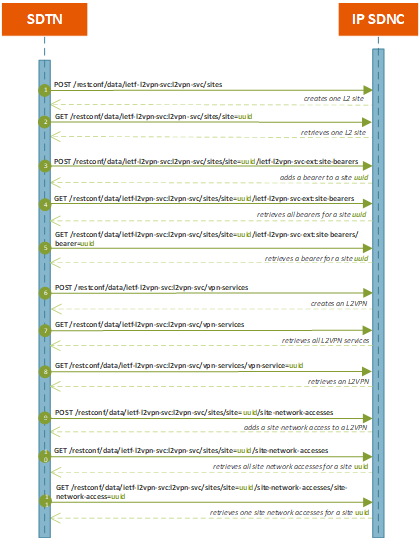
\includegraphics[width=\linewidth]{figs/l2sm_workflow_2.png}
	\caption{Messages Interchanged for L2VPN Provisioning between the SDTN and the IP SDN Controller}
	\label{FIG:L2SM_workflow}
\end{figure}

The workflow between the SDTN and the IP Controller has been summarized in the UML model presented on \cref{FIG:L2SM_workflow}. The four POST requests described previously and their equivalent GET requests exchanged between the SDTN and the IP-SDN controller are included. 

\Cref{FIG:L2SM_results} shows the L2VPN service creation results as seen from the SDTN GUI, where three information panes are included: 
\begin{itemize}
    \item Configured NEs in the network map. The yellow ones include the two service end-points.
    \item List of all the services of a common type. In this case VPLS service was selected. 
    \item Service details, including: Name, Description and End-points (vlans, ports and topology-role). 
\end{itemize}

\begin{figure}
	\centering
		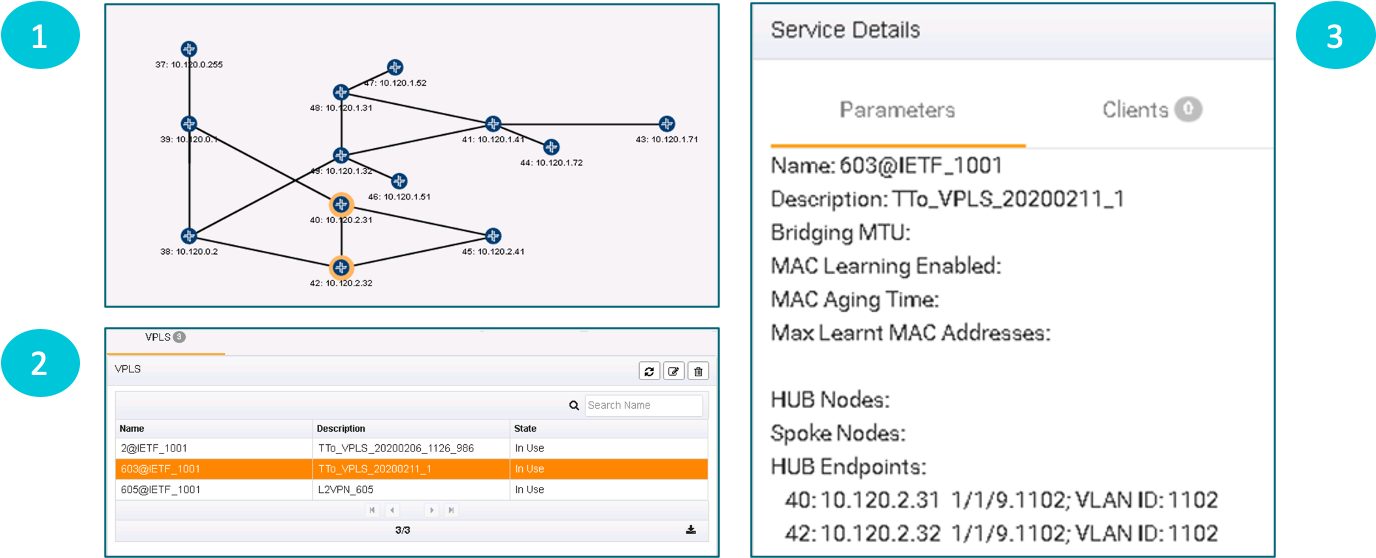
\includegraphics[width=\linewidth]{figs/l2vpn_results.png}
	\caption{L2VPN service creation results retrieved from the SDTN GUI. Information included three panes: Topology, Services lists and Service Details (Name, Topology and Endpoints).}
	\label{FIG:L2SM_results}
\end{figure}


\subsection{Multi-domain IP L3VPN provisioning}

Aiming to demonstrate the multi-domain/multi-vendor capabilities of the SDTN solution, a scenario for an L3VPN service configuration was proposed. The main goal was to create a L3VPN between two access routers, each of them located in different IP domains. The IP domains are connected using a DWDM optical network. Depicted in \cref{FIG:field_trial_optical}. The L3VPN service was created using the SDTN GUI and the configuration parameters used for this matter are shown on Table \cref{TAB:discovered_ip_l3vpn}.

\begin{table*}[]
\caption{Configuration Parameters for L3VPN}
\begin{adjustbox}{width=0.5\textwidth}
\small
\begin{tabular}{lll}
& \multicolumn{1}{c}{IP Vendor A} & \multicolumn{1}{c}{IP Vendor B} \\
{\color[HTML]{000000} NE IP Address} & {\color[HTML]{000000} 10.121.0.10}          & {\color[HTML]{000000} 10.120.1.52}     \\
\rowcolor[HTML]{F2F2F2} 
{\color[HTML]{000000} Hostname}            & {\color[HTML]{000000} 53-E114}              & {\color[HTML]{000000} 10.120.1.52}     \\
{\color[HTML]{000000} Description}         & {\color[HTML]{000000} SDTN\_TESTING-A}      & {\color[HTML]{000000} SDTN\_TESTING-B} \\
\rowcolor[HTML]{F2F2F2} 
{\color[HTML]{000000} Service   Interface} & {\color[HTML]{000000} GigabitEthernet0/2/1} & {\color[HTML]{000000} 1/1/2}           \\
{\color[HTML]{000000} IP Address}          & {\color[HTML]{000000} 10.93.234.65/29}      & {\color[HTML]{000000} 10.93.233.65/29} \\
\rowcolor[HTML]{F2F2F2} 
{\color[HTML]{000000} VLAN   ID}           & {\color[HTML]{000000} 2020}                 & {\color[HTML]{000000} 999}             \\
{\color[HTML]{000000} VLAN Mode}           & \multicolumn{2}{c}{{\color[HTML]{000000} Dot1Q}}                                     \\
\rowcolor[HTML]{F2F2F2} 
{\color[HTML]{000000} VPN   ID}            & \multicolumn{2}{c}{\cellcolor[HTML]{F2F2F2}{\color[HTML]{000000} 15}}           
\end{tabular}
\end{adjustbox}
\label{TAB:discovered_ip_l3vpn}
\end{table*}

When creating the service in a multi-domain and multi-vendor scenario, some of the  drawbacks faced were: 
\begin{itemize}
    \item Absence of data in the SDN domain controllers for an automatic inter-domain link discovery.
    \item Lack of a fully standardized model implemented in the IP SDN controllers.
    \item Differences in the maximum length size allowed on some configuration parameters (description, SNA names, etc.).
\end{itemize}

The workflow between the SDTN and the IP Controller has been summarized in the UML model presented on \cref{FIG:l3vpn_workflow}.

\begin{figure}
	\centering
		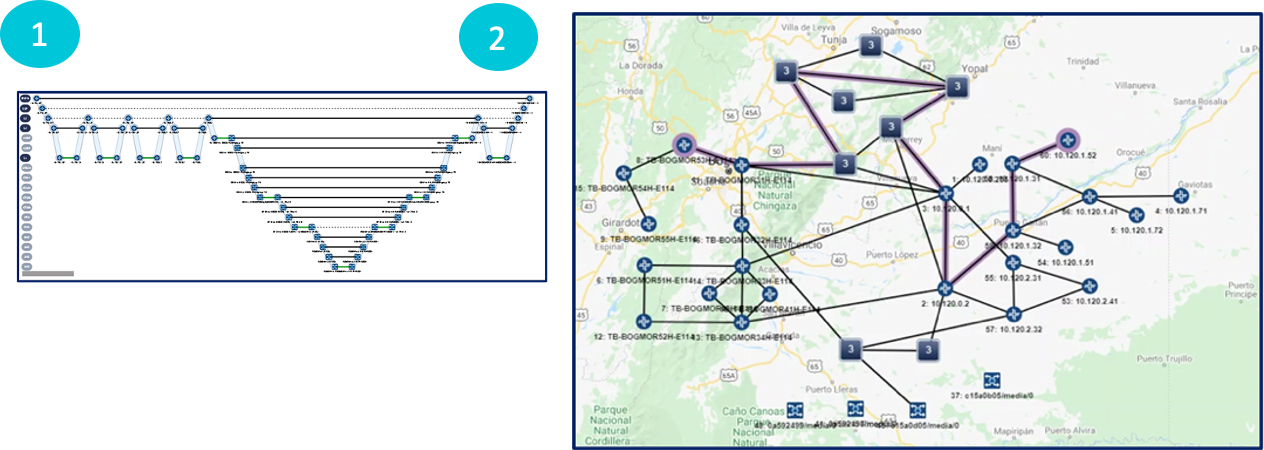
\includegraphics[width=\linewidth]{figs/l3vpn_results.png}
	\caption{L3VPN service creation results retrieved from the SDTN GUI. Included three visualization panes: The serivce details (Name, Topology, RD and Endpoints), the geographical view and the hop-by-hop connection view.}
	\label{FIG:l3vpn_results}
\end{figure}

Once these sorts of restrictions were overcome, the procedure for creating the L3VPN from the SDTN GUI was successful. \Cref{FIG:l3vpn_results} shows the two visualization options provided by the SDTN. First, a per layer view of the end-to-end IPVPN service created, or the service route as seen from the network topology view.

\begin{figure}
	\centering
		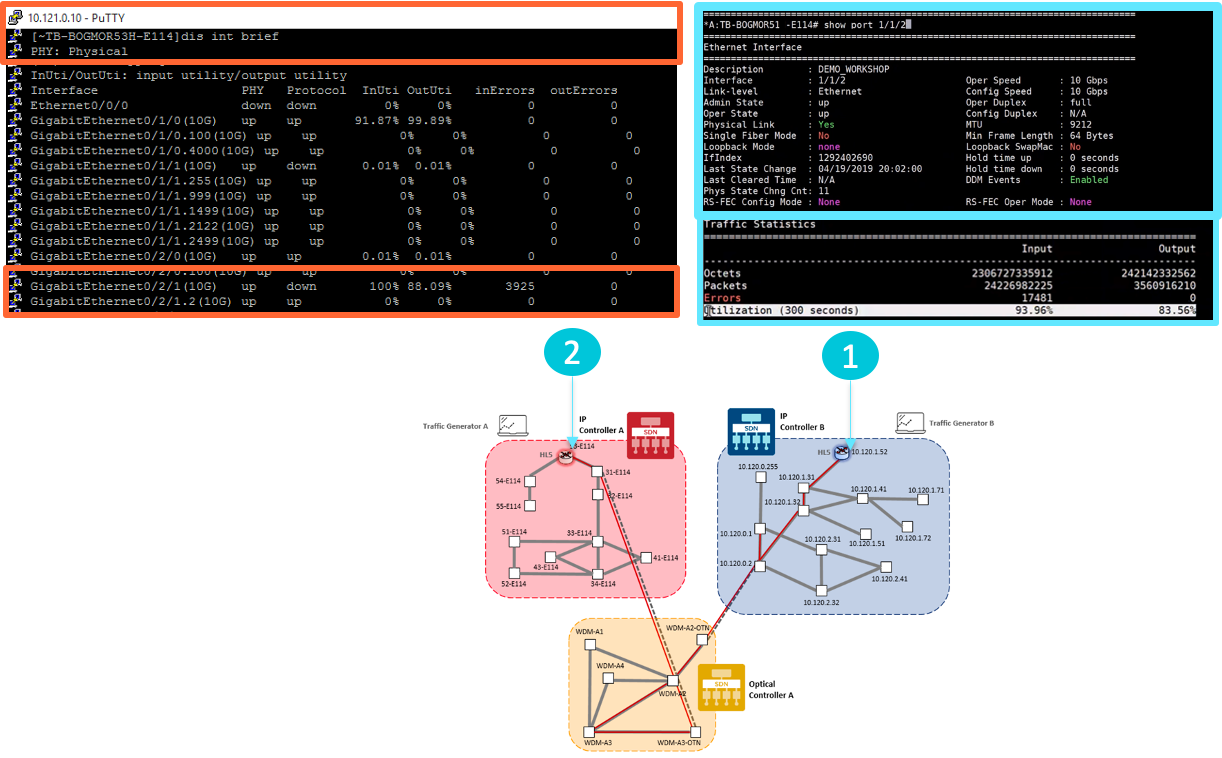
\includegraphics[width=\linewidth]{figs/counters.png}
	\caption{Traffic counters meassured on the end-points of the service. The utilization in both ends is close to 95\% due to the traffic injected by the generator.}
	\label{FIG:counters}
\end{figure}

The configuration of the IP L3VPN service in the network elements was verified by using their CLI as well as the IP-SDN controllers GUI. A traffic generator was used in site to introduce traffic on both ends of the network and test the functionality of the multi-domain L3VPN service created.\cref{FIG:counters} shows the traffic statistics as seen on the CLI of the routers.

\subsection{Optical provisioning}
From the perspective of the optical networks, single domain unconstrained DSR connectivity services as well as Photonic Media Layer services were independently configured in both vendors’ DWDM networks and were verified in the respective NMS systems. The ONF T-API 2.1 YANG data model has been used for the query exchange between the SDTN HCO and the optical domain controllers given the support of this standard model in their NBIs. The UML diagram on \Cref{FIG:optical_provisioning_workflow} shows the HTTP POST request involved in the optical circuit creation as sent from the SDTN HCO towards the Optical SDNCs, as well as the HTTP GET requests for information retrieval regarding particular connectivity services existing on the network. 

The DSR connectivity services created in both optical domains range from 1GbE, to 10GbE and 100GbE, all of them configured by using the API Client as well as the SDTN HCO GUI. A total of 3x10GbE and 4x100GbE DSR connectivity services were provisioned simultaneously on Optical Domain A whereas given the network resources available in the Optical Domain B, a 1GbE service as well as 2x10GbE services were provisioned. When it comes to photonic media type of services, 100GbE and 200GbE could be provisioned for Optical Domain A and B respectively. 

First, the API Client was used to send the E2E DSR Service creation query towards the SDNCs. For this, parameters\footnote{Parameters included in the body script for the service creation; other important ones include “service-interface-point”, “layer-protocol-name”, “service-layer” as well as the service “name” and a unique identifier “uuid”.} such as “service-interface-point”, “capacity” and “layer-protocol-qualifier” embedded in the POST body script needed to be correctly identified prior to sending the service creation petition, being that they depend strictly on the installed equipment and the resources available in the network; and therefore, when configured improperly, it led to the failure of the service creation, or to the misconfiguration on the controller’s side. When sending the POST query from the SDTN HCO towards the Optical Controllers, an HTTP 202 Accepted notification is returned by the SDNC, meaning the controller has accepted the petition and would proceed with the service creation, otherwise, an HTTP 400 Bad Request notification would be retrieved in case the petition was not accepted by the controller. 

\begin{figure}
	\centering
		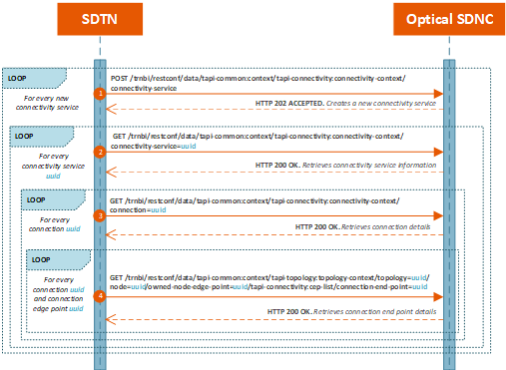
\includegraphics[width=\linewidth]{figs/optical_provisioning_workflow_2.png}
	\caption{Messages Interchanged for Optical Provisioning between the SDTN and the Optical SDN Controller}
	\label{FIG:optical_provisioning_workflow}
\end{figure}

\begin{figure}
	\centering
		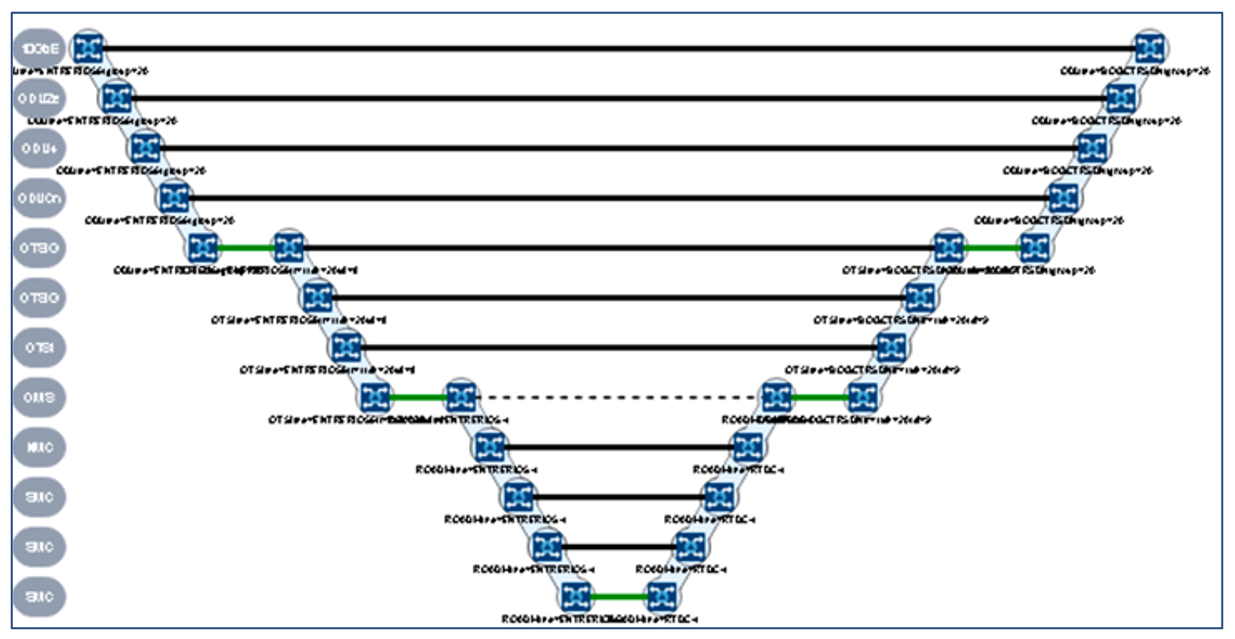
\includegraphics[width=\linewidth]{figs/optical_provisioning_result.png}
	\caption{Optical Provisioning Result for a Multi-Layer 10GbE Service}
	\label{FIG:optical_provisioning_result}
\end{figure}

Additionally, from the API client tests, it was noted that even if both controllers are standard-based and implement T-API 2.1 in their NBIs, the modelling of some attributes is different from one another. From comparing the results retrieved via the API Client, naming attributes for some of the objects\footnote{SIP\_NAME” in contrast to "INVENTORY\_ID", "CONN\_NAME" in contrast to "CONNECTION\_NAME", among others}, as well as the general modelling of the connections in regards of the route for an optical circuit was noticed to be different. Likewise, the site names in one of the optical controllers did not coincide with the real name of the site but were based on an encoding made it by the controller itself. Also, when using the SDTN HCO GUI to create the e2e connectivity services within the two network domains; this particular discrepancy was also visible via the multilayer view of the services created, as seen on \cref{FIG:optical_provisioning_workflow} where the different layers for a 1GbE service are shown as exposed by the optical domain controller B, while on \cref{FIG:optical_provisioning_result} a multilayer view of 10GbE service created on Optical Controller A is shown.


\section{Conclusions and Future Work}
\label{section:conclusions}
A key angular stone for the SDTN Architecture is the data models themselves. RESTCONF/YANG based with IETF and ONF YANG models were preferred when beginning with the integration between SDTN and the SDN-C domain controllers, the main focus was the use of a standardized API to access and retrieve the required information from the IP and Optical controllers. It is the reason behind that both Optical Domain Controllers had ONF T-API 2.1 YANG models implemented, making the integration process much easier; on the other hand, for the IP domain in particular, the usage of different pseudo-standard and reduced models was needed in order to execute the different test case scenarios. IETF YANG data models for the IP World still require additional efforts to fit in all the MPLS-based use cases as a synergy flow. 

Brief summary of faced issues during the integration of the SDTN architecture, as reference point to another work or future work: 

\begin{itemize}
    \item Connectivity, latency and internal processing times between the HCO and some of the SDN-Cs can impact the integration and result in miscommunications creaking the timeout of SDN transport protocols, ie. RESTCONF and NETCONF.  
    \item \textit{Ghost} objects which would not be completely deleted in the controllers can lead to misunderstand in the topology construction. 
    \item The unsolicited data retrieved by a lack of standardization or a bias in the implementation of the standards can lead to uncompleted transactions or loops in execution tasks. 
\end{itemize}
 However, except for the lack of the inter-domain ports exposure on the IP domains as well as the retrieval of data required for automatic discovery of Inter-Domain Links (e.g. Plug-ID and TTI values), the APIs provided sufficient functionality for their implementation of all the use cases approached on this paper, demonstrating the viability of the SDTN solution on a multi-vendor and multi-domain network environment.

\subsection{Future Work}
As future work, the hybrid SDN deployment done until now must be complemented with an integration between the NBI exposed by the SDTN and the OSS applications ecosystem. The OSS ecosystem can include for example strategic and tactical planning applications, able to support the year by year demand management and planning tasks done within the organization. A common interface defined and available for these tasks would allow the OSS systems providers to focus on the quality of the applications developed, forgetting the complexity of the network management. Economically it will generate direct reductions in the applications integration time.

Additionally, the scope of this work can be extended to cover Traffic Engineering use cases. Standardization in the NBI requests to support the LSPs creation will enable easy management of the traffic flows in the network, generating a real massification of the Traffic Engineering deployment and creating new network optimization solutions for the operators.

\printcredits

\section*{Acknowledgements}
This is work has been supported by Telefonica I+D as part of the Fusion, iFusion, and OpenFusion projects. Authors would like to thank to all the SDN technical teams and leaders that participate in the development, deployment, and testing of this SDTN architecture. Many thanks for their contributions to Manuel Santiago, Gloria Gomez, Julia Rodriguez and  Stevkovski from Infinera, Randy Quimbay, David Rocha from Telefonica Colombia, and Andrea Valencia, Juan Suarez, Juan Agredo and Daniel Hernandez from Wipro.   

%% Loading bibliography style file
%\bibliographystyle{model1-num-names}
%\bibliographystyle{cas-model2-names}
\bibliographystyle{ieeetr}

% Loading bibliography database
\bibliography{bibliography}


%\vskip3pt

\bio{figs/1010179793S.jpg}
Phd Candidate.
\endbio

\bio{}
Author biography with author photo.
\endbio

\bio{}
Author biography with author photo.
\endbio

\end{document}

